% !TEX program = xelatex

\documentclass[titlepage]{article}

\usepackage{geometry}

\usepackage{polyglossia}
\setdefaultlanguage{greek}
\setotherlanguage{english}

\usepackage{fontspec}
\setmainfont{Noto Serif}
\setsansfont{Noto Sans}
\setmonofont{Noto Mono}
\newfontfamily\greekfont{Noto Serif}
\newfontfamily\greekfontsf{Noto Sans}
\newfontfamily\greekfonttt{Noto Mono}

\usepackage{graphicx}
\graphicspath{{../plots/}}
\usepackage{subcaption}

\usepackage{amsmath}

\begin{document}

\title{Γλώσσες Προγραμματισμού II\\
    Άσκηση 6}
\author{Αλέξιος Ζαμάνης\\
    03115010}

\maketitle

\section*{Παραλληλισμός και ταυτοχρονισμός στη Haskell}

Στα πλαίσια της άσκησης υλοποιούμε έναν αποδοτικό αλγόριθμο υπολογισμού του διωνυμικού συντελεστή. Στη συνέχεια υλοποιούμε διάφορες παράλληλες εκδόσεις του αλγορίθμου χρήσει 2 βιβλιοθηκών παράλληλου προγραμματισμού της Haskell. Εν τέλει εκτελούμε μια σειρά από μετρήσεις και εκτιμούμε την κλιμακωσιμότητα των υλοποιήσεών μας βάσει της επιτάχυνσης που επιτυγχάνουν.

\subsection*{Διωνυμικός συντελεστής}

Καλούμαστε να υπολογίσουμε έναν διωνυμικό συντελεστή modulo έναν πρώτο αριθμό $p$. Ζητάμε δηλαδή την τιμή της παράστασης ${n\choose k}\mod p$ για δεδομένους μη αρνητικούς ακεραίους $n, k, p$.

\paragraph{Βασικές ιδιότητες}

Δίνεται ότι $k\leq n$. Συνεπώς έχουμε ότι ${n\choose k}=\frac{n!}{k!(n-k)!}=\frac{n\dots(n-k+1)}{k!}$. Βλέπουμε εύκολα ότι ισχυέι η ιδιότητα ${n\choose k}={n\choose n-k}$. Επομένως φροντίζουμε πάντα να υπολογίζουμε βάσει του μικρότερου εκ των $k$ και $n-k$. Επιπλέον γνωρίζουμε ότι $ab\mod n=(a\mod n)(b\mod n)\mod n$. Η ιδιότητα αυτή είναι αναγκαία, ώστε να αποφύγουμε τις υπερχειλίσεις κατά τον υπολογισμό του διωνυμικού συντελεστή για μεγάλα $n$ και $k$.

\paragraph{Το μικρό θεώρημα του Fermat}

Για να αξιοποιήσουμε την παραπάνω ιδιότητα του πολλαπλασιασμού, απαιτείται να υπολογίσουμε τον αντίστροφο του $k!$ modulo $p$. Σύμφωνα με το θεώρημα του Fermat, για έναν πρώτο p ισχύει $a^p=a\mod p$. Δίνεται όμως ότι $k<p$. Επομενως τα $k$ και $p$ δεν έχουν μη τετριμμένο κοινό πολλαπλάσιο, οπότε ισχύει ότι $(k!)^{-1}=(k!)^{p-1}\mod p$. Ο υπολογισμός του αντιστρόφου ανάγεται επομένως στον υπολογισμό μιας δύναμης modulo $p$, που επιτυγχάνεται σε λογαριθμικό χρόνο με αλλεπάλληλους τετραγωνισμούς.

\subsection*{Παράλληλη υλοποίηση}

Για να βελτιώσουμε την επίδοση της υλοποίησής μας σε πολυπύρηνους επεξεργαστές, σπάμε τον αλγόριθμό μας σε εργασίες που μπορούν να εκτελεστούν παράλληλα. Στη συνέχεια χρησιμοποιούμε τις κατάλληλες βιβλιοθήκες, ώστε να αναθέσουμε την παράλληλη εκτέλεση των εργασιών αυτών σε όσο το δυνατόν περισσότερους πυρήνες.

\paragraph{Ο παραλληλισμός στον αλγόριθμο}

O υπολογισμός του διωνυμικού συντελεστή συνίσταται στον υπολογισμό του αριθμητή και του αντιστρόφου του παρανομαστή και στον πολλαπλασιασμό αυτών. Οι δύο εργασίες είναι πλήρως ανεξάρτητες, οπότε μπορούν να εκτελεστούν παράλληλα. Ο υπολογισμός του αριθμητή και του παρανομαστή μπορούν να παραλληλοποιηθούν περαιτέρω, καθώς ανάγονται στον υπολογισμό του γινομένου των αριθμών εντός ενός διαστήματος. Σπάμε επομένως το διάστημα σε ένα ορισμένο πλήθος υποδιαστημάτων, υπολογίζουμε το καθένα χωριστά και πολλαπλασιάζουμε τα επιμέρους γινόμενα. Έχουμε δηλαδή ένα reduction. Διακρίνουμε λοιπόν δύο επίπεδα παραλληλίας. Σημειώνουμε εδώ ότι δεν παραλληλοποιούμε τον υπολογισμό του αντιστρόφου, καθώς κάθε βήμα εξαρτάται από το προηγούμενό του, οπότε δεν έχουμε παραλληλία. Άλλωστε ο αλγόριθμος ύψωσης σε δύναμη είναι λογαριθμικός, έναντι των προαναφερθέντων πολλαπλασιαμών που είναι γραμμικοί.

\paragraph{Ο παραλληλισμός στο δοθέν πρόβλημα}

Στη δοθείσα διατύπωση του προβλήματος καλούμαστε να υπολογίσουμε T το πλήθος διωνυμικούς συντελεστές για ένα δοθέν T. Προφανώς κάθε διωνυμικός συντελεστής μπορεί να υπολογισθεί τελειώς ανεξάρτητα από τους υπόλοιπους και παράλληλα με αυτούς. Επομένως, πέραν των παραπάνω επιπέδων παραλληλίας, υπάρχει ένα ακόμα τέλεια παραλληλοποιήσιμο επίπεδο.

\paragraph{Οι βιβλιοθήκες parallel και monad-par}

Για την υλοποίηση της παραλληλοποίησης σε Haskell χρησιμοποιούμε τις βιβλιοθήκες parallel και monad-par, καθώς και διάφορες έτοιμες συναρτήσεις που έχουν υλοποιηθεί πάνω από αυτές. Από άποψη προγραμματιστικής ευκολίας η βιβλιοθήκη parallel είναι πληρέστερη και ευκολότερη στη χρήση, αν και απαιτεί μια στοιχειώδη κατανόηση των εννοιών της οκνηρής αποτίμησης. Στο κώδικα που παρατίθεται σημειώνεται με σχόλια το τμήμα κώδικα που αντιστοιχεί στην υλοποίηση με την εκάστοτε βιβλιοθήκη.

\subsection*{Πειράματα}

Για την αξιολόγηση των υλοποιήσεών μας εκτελούμε μια σειρά από πειράματα. Από τα αποτελέσματα που λαμβάνουμε υπολογίζουμε την επιτάχυνση που επιτύχαμε για ολοένα αυξανόμενο πλήθος πυρήνων και εκτιμούμε έτσι την κλιμακωσιμότητα κάθε υλοποίησης.

\paragraph{Περιγραφή των πειραμάτων}

Τα πειράματα εκτελούνται σε επεξεργαστή με 4 φυσικούς πυρήνες, που χάρη στην τεχνολογία hyper-threading φαίνονται ως 8 εικονικοί πυρήνες. Επομένως εκτελούμε μετρήσεις με 1, 2, 4 ή 8 πυρήνες. Προφανώς για 1 πυρήνα έχουμε σειριακή εκτέλεση. Επιπλέον μεταβάλλουμε την παράμετρο T του προβλήματος, ήτοι το πλήθος των ερωτημάτων, δοκιμάζοντας τιμές στο διάστημα από 1 έως και 1024. Για να είναι σταθερή η δυσκολία του δοθέντος προβλήματος ανεξαρτήτως του T, φροντίζουμε να παράγουμε τυχαίες εισόδους που κατανέμονται ομοιόμορφα στο εύρος που καθορίζει το πρόβλημα. Επιπλέον φροντίζουμε να παράγουμε πάντα την ίδια είσοδο για δεδομένο T.

\paragraph{Αποτελέσματα}

Τα αποτελέσματα των μετρήσεων φαίνονται στα κάτωθι σχήματα. Συγκεκριμένα στο σχήμα 1 βλέπουμε το χρόνο εκτέλεσης για κάθε υλοποίηση και συνδυασμό παραμέτρων, ενω στο σχήμα 2 βλέπουμε την αντίστοιχη επιτάχυνση, ήτοι το χρόνο κανονικοποιημένο ως προς το χρόνο της αντίστοιχης σειριακής εκτέλεσης.

\begin{figure}[!ht]
    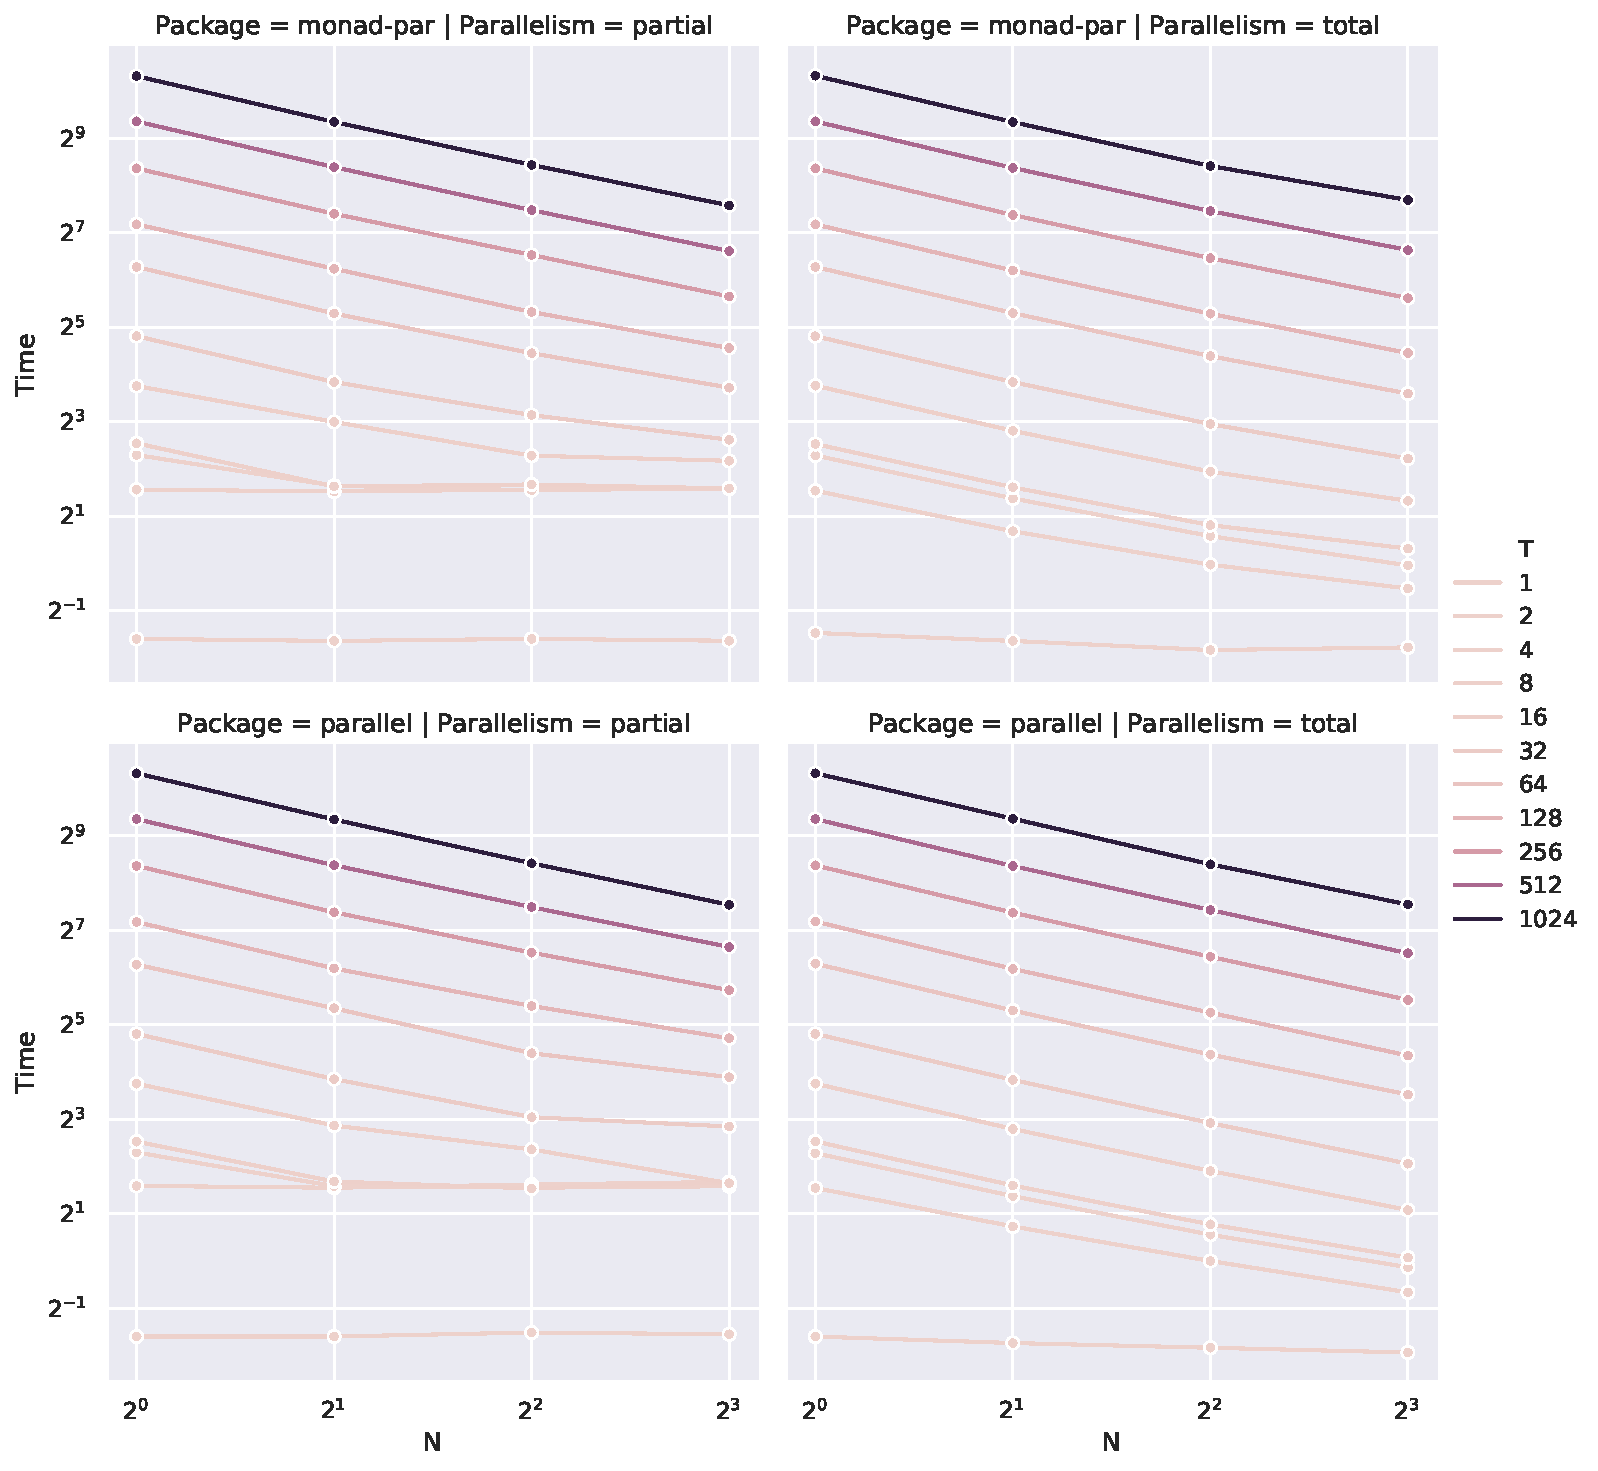
\includegraphics[width=\textwidth]{time.pdf}
    \caption{Χρόνος}
\end{figure}

\begin{figure}[!ht]
    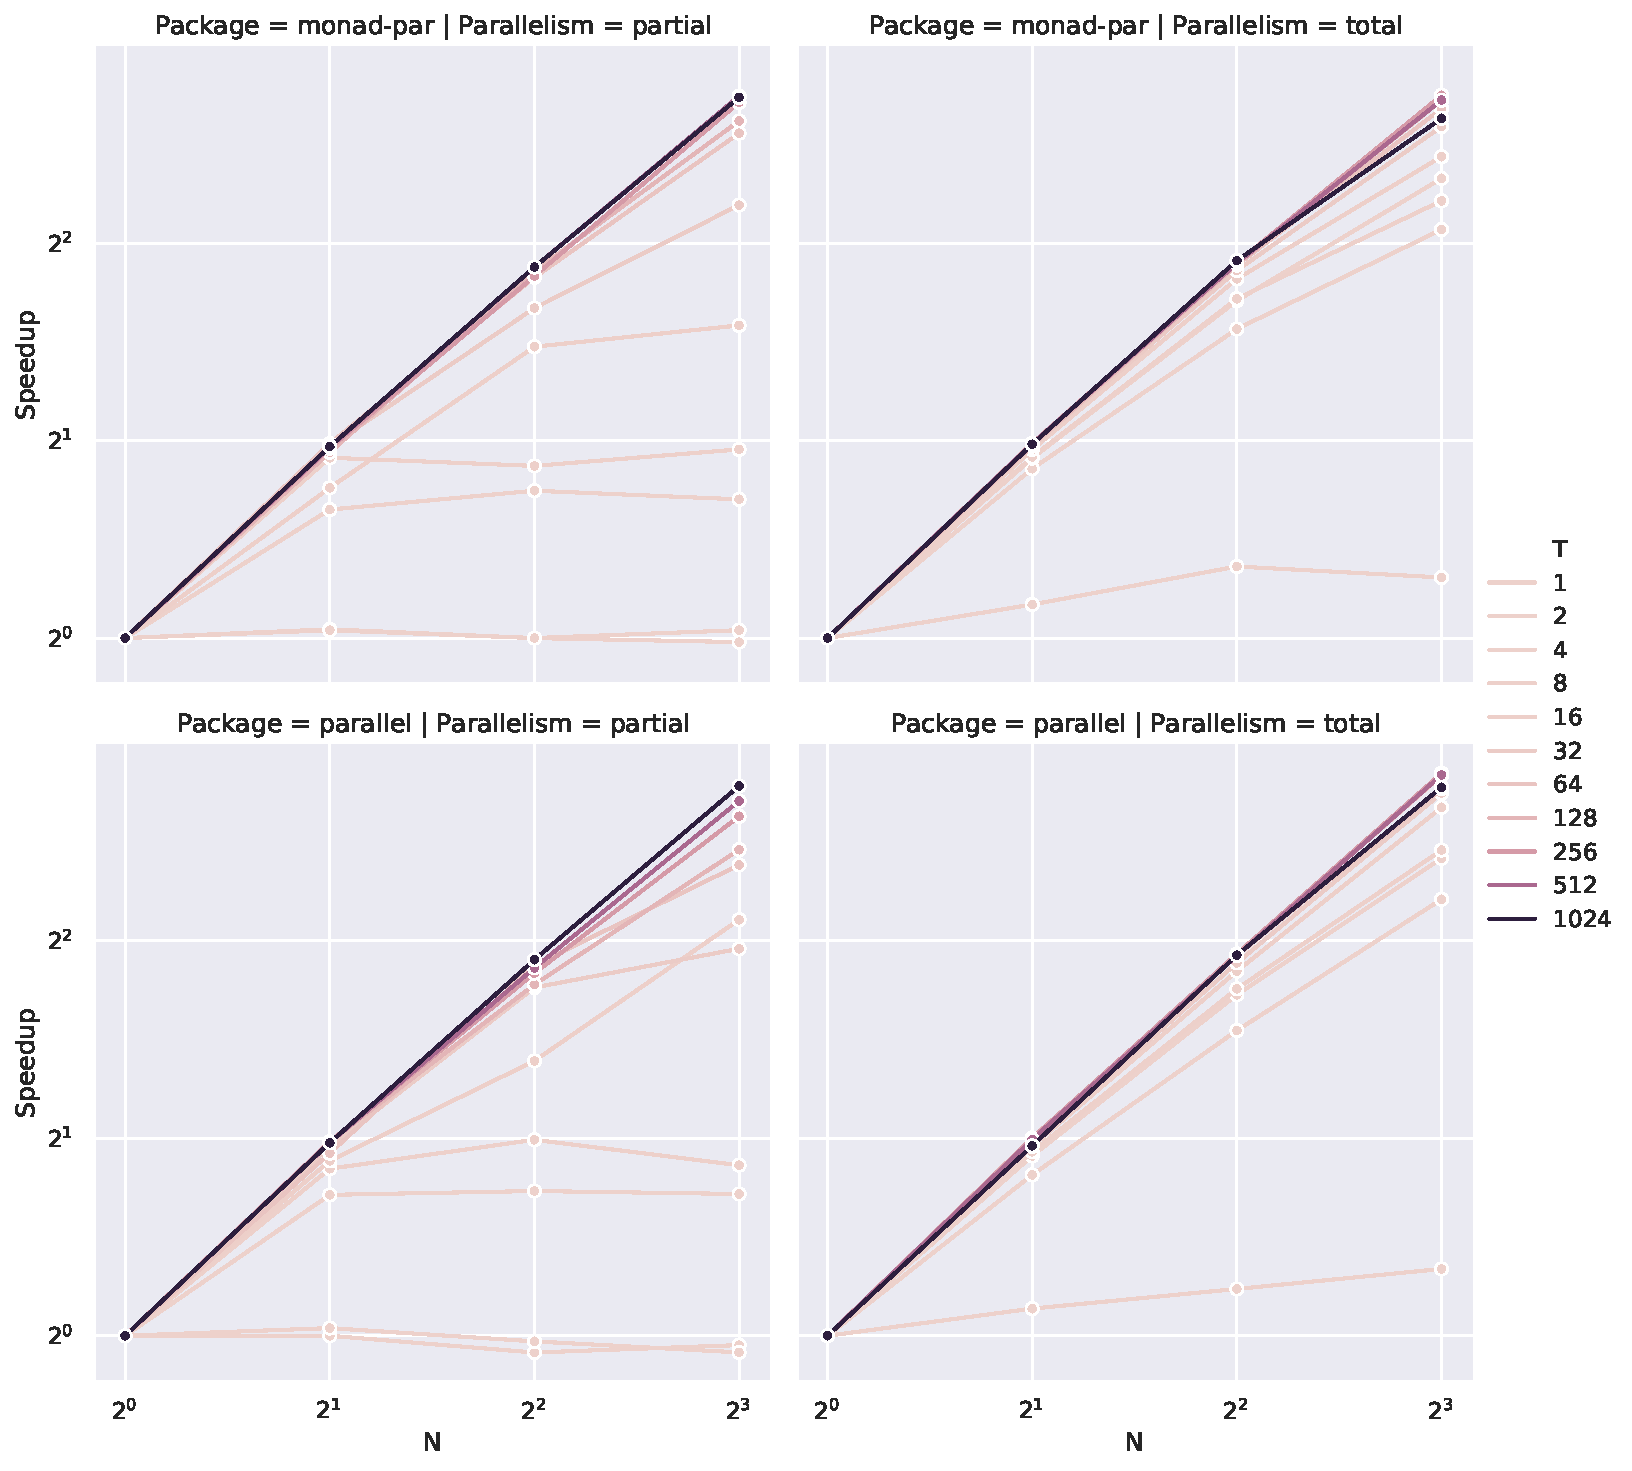
\includegraphics[width=\textwidth]{speedup.pdf}
    \caption{Επιτάχυνση}
\end{figure}

\paragraph{Κλιμάκωση}

Αρχικά παρατηρούμε με μεγάλη ευχαρίστηση ότι όλες οι υλοποιήσεις μας κλιμακώνουν. Βλέπουμε ότι έχουμε επιτύχει γραμμική ή σχεδόν γραμμική επιτάχυνση. Για 2 πυρήνες έχουμε πετύχει επιτάχυνση 2, ήτοι τέλεια κλιμάκωση. Για 4 και 8 πυρήνες έχουμε κατά μέγιστο επιτάχυνση 3.8 και 7.2 αντίστοιχα. Προφανώς κλιμάκωση 8 για 8 πυρήνες δεν είναι εφικτή, δεδομένου ότι πρόκειται για εικονικούς πυρήνες, επομένως δικαιούμαστε να θεωρήσουμε την κλιμάκωση που επιτύχαμε σχεδόν τέλεια.

\paragraph{Η επίδραση του πλήθους των ερωτημάτων}

Είναι σαφές ότι η αύξηση του πλήθους των ερωτημάτων ευνοεί την κλιμάκωση του συστήματος. Όλες οι υλοποιήσεις μας παραλληλοποιούν τα ερωτήματα, επομένως μεγαλύτερο πλήθος ερωτημάτων σημαίνει ότι λιγότεροι πυρήνες θα μένουν άεργοι, είτε επειδή έλαβαν λιγότερα ερωτήματα είτε επειδή τα ερωτήματά τους έτυχε να είναι ευκολότερα. Ήτοι για περισσότερα ερωτήματα έχουμε καλύτερη εξισορρόπηση του φορτίου, επομένως καλύτερη κλιμάκωση. Στην πράξη βλέπουμε ότι για 256 ερωτήματα και πάνω έχουμε ικανοποιητική κλιμάκωση και για 8 πυρήνες, ακόμα και στην περίπτωση που παραλληλοποιούμε μόνο τα ερωτήματα.

\paragraph{Η επίδραση του βαθμού παραλληλισμού}

Η εξάρτηση από το πλήθος των ερωτημάτων μπορεί να μειωθεί αισθητά αυξάνοντας το βαθμό παραλληλισμού. Παραλληλοποιώντας επιπλέον τον ίδιο τον αλγόριθμο, ήτοι παραλληλοποιώντας εσωτερικά κάθε ερώτημα, καταφέρνουμε πλέον να έχουμε ικανοποιητική κλιμάκωση στους 8 πυρήνες για τιμές του T από 32 και πάνω. Σημειώνουμε ωστόσο ότι υπάρχει μια τιμή του βαθμού παραλληλισμού, πάνω από την οποία το κόστος της διαχείρισης των εργασιών αρχίζει να υπερβαίνει τα οφέλη του παραλληλισμού. Εν προκειμένω παρατηρούμε ότι για 1024 ερωτήματα αμφότερες οι πλήρως παραλληλοποιημένες υλοποιήσεις αποδίδουν χειρότερα από τις αντίστοιχες μερικώς παραλληλοποιημένες.

\paragraph{Η επίδραση της βιβλιοθήκης}

Η συμπεριφορά που παρουσιάζει η υλοποίηση χρήσει της βιβλιοθήκης parallel είναι ιδιαίτερα όμοια με αυτήν της υλοποίησης χρήσει της monad-par. Ωστόσο η βιβλιοθήκη parallel φαίνεται να έχει επιτύχει καλύτερους χρόνους και επιταχύνσεις. Επομένως προτιμητέα δείχνει να είναι η χρήση της βιβλιοθήκης parallel. Σημειώνουμε ωστόσο ότι για παραλληλοποίηση μόνο των ερωτημάτων η monad-par επιτυγχάνει εν γένει καλύτερους χρόνους από την parallel. Επομένως μπορούμε να συμπεράνουμε πως η monad-par ευνοείται από coarse-grained υλοποιήσεις, ενώ η parallel αριστεύει σε fine-grained υλοποιήσεις.

\end{document}
